\documentclass[12pt]{article}
\usepackage[a4paper, margin=1in]{geometry}
\usepackage{lmodern}
\usepackage{graphicx} % Required for inserting images
\usepackage{ucs}
\usepackage{notoccite}
\usepackage{float}
\usepackage{svg}
\svgsetup{inkscapeexe=inkscape}
\svgpath{{./Images/}}  % Set the path for SVGs
\usepackage{amsmath}
\usepackage{hyperref} % For clickable links
\graphicspath{{./Images/}}

\hypersetup{
    colorlinks=true,       % false: boxed links; true: colored links
    linkcolor=blue,        % color of internal links
    citecolor=blue,        % color of links to bibliography
    filecolor=magenta,     % color of file links
    urlcolor=cyan          % color of external links
}


\begin{document}


\section{VA001}
VA001 is a Basic self bias Miller Operational transcondutance amplifier, exemplified in Fig. \ref{VA001}.


%O start up esta mau, tem de ser alterado
\begin{figure}[H]
        \centering
        \includesvg[width=1\textwidth]{VA001.svg}
        \caption{proposed self bias two stage operational transcondutance amplifier.}
        \label{VA001}
\end{figure}
\subsection{Circuit explanation}
$P_1 - P_2$, $N_1 - N_4$, and $R_1$ form the biasing cell, functioning as a PTAT current bias generator.  

The proportional relationship comes from $N_3$ having a transconductance four times lower than that of $N_4$. As temperature increases, $V_{GS_3}$ rises, which increases the current through $N_4$ due to its higher transconductance, as both gates are connected. The current mirrors formed by $P_1$ and $P_2$ ensure equal currents, establishing an internal feedback loop. Transistors $N_1$ and $N_2$ limit the voltage across $N_3$ and $N_4$, thereby improving the PSRR. Additionally, $R_1$ introduces degeneration in $N_4$, allowing for better control over the reference current and transconductance.

To maximize PSRR and minimize unwanted feedback from the amplifier to the bias cell, the transistor sizes should not be excessively large, but minimum size transistors should be avoided at all cost, transistor with L or W close to the minimum size have a current curve with very prominent short channel effects that can impact a circuit very negatively, suffer more from hot carrier degradation and are very susceptible to random variation during fabrication. 


By assuming an initial condition of $V_{IN+} = V_{IN-} = V_{DD}/2$ every node in the circuit is fixed at some DC voltage value.  theoretical its assumed that $V_{OUT}=V_{DD}/2$ in this condition.
Focusing on the first stage, a change in $V_{IN+}$ equal to $\Delta V_{IN+}$ occurs leading to a symmetric current change of $-\Delta I_{PAIR+} = \Delta I_{PAIR-}$. This current change is expressed as $-\Delta I_{PAIR+} = \Delta V_{IN+} \times g_{mP6}$. Ignoring the current source $P_5$, the output variation of the first stage can be described as $-\Delta V_{IN+} \times g_{mP5} (R_{oP5} \parallel R_{oN6})$, where $g_{mP5} = g_{mP6}$ and the small-signal output impedance is the parallel combination of the output impedance's of $P_6$ and $N_6$.




Since $N_5$ is diode-connected, the current variation $\Delta I_{PAIR-}$ causes a corresponding $\Delta V_{GS_{N5}}$, which is proportional to $\Delta V_{IN+} \times g_{mP5}  \times R_{oN5}$.  Because $N_6$ shares the same gate potential, its output impedance inversely varies with $\Delta V_{IN+}$,  leading to a gain variation with $\Delta V_{IN+}$. While this typically poses no issue in a closed-loop configuration and a relatively small signal amplification, where the gain is stabilized by feedback, this variation introduces significant distortion in the output signal in open-loop configurations.


Since \( V_{\text{DS}_{N6}} = V_{\text{GS}_{N8}} \), any variation at this node is subsequently amplified through a common-source amplifier in the second stage. Assuming that \( P_4 \) remains in saturation during steady-state operation, \( I_{\text{BIAS2}} \) is considered constant, with channel-length modulation effects being negligible. Given that the second-stage input transistor \( N_8 \) also operates in saturation under steady-state conditions, any change in \( V_{\text{GS}_{N8}} \) induces a significant variation in \( V_{\text{DS}_{N8}} \), or equivalently, \( V_{\text{OUT}} \).  This variation can be quantified as \( -g_{\text{m}_{N8}} \left( R_{\text{o}_{P4}} \parallel R_{\text{o}_{N8}} \right) \).

Since the gain of the common-source amplifier is inherently negative, the overall multiplication of the gains from the two amplifier stages results in a \(\Delta V_{\text{OUT}}\) that is directly proportional to \(\Delta V_{\text{IN+}}\), with the amplifier gain expressed as

\begin{equation}
A_d \approx  g_{mP5}(R_{0P5}//R_{0N6})\times g_{mN8}(R_{0P4}//R_{0N8}).
\label{gainnnn}
\end{equation}



Due to its structure, the second stage provides a significantly larger output swing than the previous stage while maintaining a similar gain. However, since the gain is absolute rather than differential, using it alone makes it more susceptible to distorted output signals. 


This amplifier is significantly affected by input CMV variations, as it lacks an auxiliary circuit to regulate it. The common-mode variation originates from changes in $I_{bias1}$ as a function of the input CMV. When the common-mode voltage fluctuates, the $V_{DS}$ of the input differential pair also changes, leading to a voltage shift at the common node of the input pair. 

This shift induces a $\Delta I_{bias1}$, which depends on the output impedance of the current source and is influenced by the channel-length modulation parameter, $\lambda$.
Since the DC output voltage is largely determined by the bias current when $I_{PAIR+} = I_{PAIR-}$, any changes in the input CMV result in variations in the output voltage. This variation depends on the impedance of the differential pair and the active load. The CMRR quantifies the amplifier’s ability to reject common-mode signals, and it is defined as the ratio between the differential gain and the common-mode gain.

The CMRR expression can be expressed as
\begin{equation}
CMRR \approx \frac{A_d}{A_c} = 2(g_{m_P5}+g_{m_N2})*(R_{0_N2}+R_{0_P5})R_{0_P3}.
\label{gasdsdd}
\end{equation}
CMRR is an important metric that indicates how effectively the amplifier rejects common-mode noise. It is highly dependent on the output impedance of the current mirror used to bias the amplifier, as shown in Eq.\ref{gasdsdd}. CMRR is also closely related to THD since it is directly influenced by $\Delta I_{bias1}$ as a function of $\Delta V_{DS}$ of the input transistors, which naturally vary during normal signal amplification. As with other amplifiers, the primary noise sources are typically the current sources and the differential pair. To mitigate noise, transistors $P_3$ and $P_4$ should not have excessively low transconductance or be too small in size. Additionally, minimizing noise requires the differential pair to have a relatively high transconductance.
As with previous amplifiers, the primary noise sources are typically associated with the current sources and the differential pair. This case is no different. To mitigate noise, $P_3$ and $P_4$ should have a low transconductance nor be sized too small. Additionally, to further minimize noise, the differential pair should have a relatively high transconductance.


Instability occurs when the first stage of an amplifier responds faster than the output stage. To mitigate this, a compensation network is introduced, using Miller compensation to slow down the first stage’s response. This technique achieves pole splitting, where the dominant input pole is shifted closer to the right half-plane, while the output pole is moved to the left half-plane, enhancing stability. However, this comes at the cost of reduced bandwidth and increased capacitor and resistor sizes. Additionally, ensuring that the bias current of the second stage ($I_{BIAS2}$) is larger than that of the first stage helps to space the two poles apart, further improving stability naturally. Without a compensation circuit, the bias current of the second stage would need to be extremely high for a stable system, leading to inefficiency in power consumption. The compensation network is formed by $C_C$ and $P_8$.

\subsection{Design methodology}

To size the transconductance cell, $I_{REF}$ can be determined as follows:

\begin{equation} I_{REF} = \frac{2}{C_{ox} \cdot \mu_n \cdot \frac{W_{N_{4}}}{L_{N_{4}}}} \cdot \frac{1}{R_1^2} \cdot \left(\frac{1}{\sqrt{k}}\right)^2, \label{eq
} \end{equation}

where $k=4$ as explained.

The PMOS transistor current mirror should be sized to achieve the desired voltage overdrive for a given bias current. In this case, the initial $I_{REF}$ was chosen to be $5\ \mu A$. A common rule of thumb when designing current mirrors is to start with an overdrive voltage ($OV_{P1}$) of around 200 mV. The following equation can be used as a reference to aid in sizing the PMOS transistors:

\begin{equation} OV_{P1} = \sqrt{\frac{2 \cdot I_{BIAS}}{\mu_{P} \cdot C_{ox} \cdot \frac{W_{P1}}{L_{P1}}}}. \end{equation}

To further aid in selecting the overdrive voltage of the {PMOS} current mirror, the ICMR can be expressed as:

\begin{equation} I_{CMR} = V_{DD} - OV_{P3} - VTH_{P1}, \end{equation}

with $OV_{P1} = OV_{P2} = OV_{P3} = OV_{P4}$.

Temperature sweeps should be performed to observe how the reference current changes with temperature. The sizes of $N_1 - N_4$ should be adjusted to obtain the desired temperature/current relationship, and the resistor should be sized to achieve the desired $I_{REF}$ value.

In the first and second stages, a good starting point is sizing $P_3$ to have four times the transistors of $P_1$, leading to a bias current ($I_{bias}$) that is four times the reference current ($I_{REF}$). For $P_4$, a good starting point is twice the size of $P_3$ to increase the distance between the input pole and the output pole, improving stability and the slew rate of the amplifier.

Now, observing the compensation network, the gain bandwidth with Miller compensation of the amplifier can be expressed as:

\begin{equation} GBW = A_d \cdot \omega_{pI} \approx \frac{g_{mP4}}{C_C}. \end{equation}

Since the transconductance can be expressed as:

\begin{equation} g_m = \frac{2 \cdot I_D}{V_{GS} - V_{TH}}, \end{equation}

the gain bandwidth is directly dependent on the relationship between the first-stage bias current and the value of the compensation capacitor in the compensation network. 

Therefore, the bias current and the compensation capacitor should be chosen such that, even in the worst-case scenario, the amplifier maintains a UGBW larger than the minimum required UGBW.

Another important factor is the zero introduced by $N_7$. To save space, a transistor in the triode region is used instead of a resistor, which is a trade-off between linearity and space savings. By introducing a well-placed zero, the phase margin can be improved. The zero can be expressed as:

\begin{equation} \omega_z = \frac{1}{\left(\frac{1}{g_{mN8}} - R_{0N7}\right)C_C}. \end{equation}

The location of the output dominant pole can be expressed as:

\begin{equation} \omega_{pO} = \frac{g_{mN8}}{C_L}. \end{equation}

Parametric simulations, based on the previously shown equations, should be performed to size the two stages with the compensation network, considering bandwidth, gain, phase margin, and the desired slew rate. If an increase in bias current is required, the resistor of the transconductance cell should be reduced rather than adjusting the ratio of fingers of $P_3$ and $P_4$, to maintain layout symmetry.


\newpage

\section{VA002}
VA002 is a two stage amplifier with some different tricks, shown in Fig. \ref{VA002}.
\begin{figure}[H]
        \centering
        \includesvg[width=1\textwidth]{VA002.drawio.svg}
        \caption{proposed self bias two stage operational transcondutance amplifier.}
        \label{VA002}
\end{figure}
\subsection{Circuit explanation}
$P_1 - P_2$, $N_1 - N_4$, and $R_1$ form the biasing cell, functioning as a PTAT current bias generator.  The transcondutance cell is a variation off the previously used transcondutance cell.

The proportional relationship comes from $N_3$ having a transconductance four times lower than that of $N_4$. As temperature increases, $V_{GS_3}$ rises, which increases the current through $N_4$ due to its higher transconductance, as both gates are connected. The current mirrors formed by $P_1$ and $P_2$ ensure equal currents, establishing an internal feedback loop. Transistors $N_1$ and $N_2$ limit the voltage across $N_3$ and $N_4$, thereby improving the PSRR. Additionally, $R_1$ introduces degeneration in $N_4$, allowing for better control over the reference current and transconductance.

$P_3$ and $N_5-N_6$ form the $I_{ref_2}$ current generator. The generated $I_{BIAS1}$ is approximately dependent on $I_{PTAT} \cdot k_1$, where $k$ is the size ratio between $N_5$ and $N_2$. The benefit of this approach is that it simplifies scaling the bias of the gain stage in relation to the PTAT generator. Usually, the smaller the current of the transconductance, the better the linearity, though this is a niche case. $P_{10}-P_{11}$, $R_2$, and $N_{12}$ form the $I_{ref_3}$ generator. This configuration generates a low voltage swing current, which increases the current swing of the transistors without impacting the generation of the reference current. $P_6-P_9$ and $N_7-N_{11}$ form the first stage.  By assuming an initial condition of $V_{IN+} = V_{IN-} = V_{DD}/2$, every node in the circuit is fixed at some DC voltage value. Theoretically, it is assumed that $V_{OUT} = V_{DD}/2$ under this condition. Focusing on the first stage, a change in $V_{IN+}$ equal to $\Delta V_{IN+}$ leads to a symmetric current change of $\Delta I_{PAIR+} = -\Delta I_{PAIR-} = -\Delta I_{P_7} = \Delta V_{IN+} \cdot g_{mN8}$. This allows the variation in the first stage to be expressed as: \[ \Delta V_{OUT_1} = -\Delta V_{IN+} \times g_{mN8} \times \left( ((R_{oN_{8}} \parallel R_{oP7}) g_{mP_9} R_{oP9}) \parallel R_{oN11} \right), \] This happens because the impedance of the PMOS current source is in parallel with the impedance of the differential pair. Then, the impedance in combination with the transconductance of $P_9$ can be considered in series, with the entire configuration being in parallel with $N_{11}$.  Since $N_{10}$ is diode-connected, the current variation $\Delta I_{PAIR-}$ causes a corresponding $\Delta V_{GS_{N5}}$, which is proportional to $-\Delta V_{IN+} \times g_{mN5} \times R_{oN10}$. Because $N_{11}$ shares the same gate potential, its output impedance inversely varies with $\Delta V_{IN+}$, leading to a gain variation with $\Delta V_{IN+}$. 

While this generally poses no issue in closed-loop configurations with small-signal amplification (where the gain is stabilized by feedback), this variation introduces significant distortion in open-loop configurations. Since $V_{DS_{N11}} = V_{GS_{N14}}$, the variation is further amplified through a common-source amplifier in the second stage. Assuming that $P_4$ remains in saturation during steady-state operation, $I_{BIAS2}$ is considered constant, neglecting channel-length modulation effects. Given that the input transistor of the second stage, $N_8$, is also saturated in steady state, any change in $V_{GS_{N8}}$ leads to a significant variation in $V_{DS_{N8}}$, or equivalently, $V_{OUT}$. This variation can be expressed as $-g_{mN14}(R_{oP11} \parallel R_{N_{14}})$. 

The gain equation can be expressed as: \[ A_{V} = g_{mN8} \times \left( ((R_{oN8} \parallel R_{oP7}) g_{mP9} RO_{P_{9}}) \parallel R_{oN11} \right) \times g_{mN14} (R_{oP11} \parallel R_{oN14}), \] Because the first stage is a cascode stage, the gain of this amplifier is very high and will generally have and higher slew rate. However, the trade-off is that, due to the larger number of transistors, it will have lower bandwidth for the same current because of the parasitic capacitance that each transistor add in the signal path. Additionally, the output voltage swing of the first stage is limited, as all transistors in a cascode stage need to remain in saturation.

\subsection{Design methodology}
Usually, for good sizing, the most important choice is the relation between $I_{BIAS1}$, $I_{Pair}$, and $I_D$. Typically, the safest option is $I_{Pair} = I_D = \frac{I_{BIAS1}}{2}$, or a fifty-fifty relation. Increasing the current in the differential pair will increase the transconductance of the differential pair, but it will also reduce the output impedance of the amplifier, while limiting the swing of the amplifier. Usually, the safest option is to maintain this balance. For the $I_{BIAS1}$ generator, the transistors should be sized to obtain the desired voltage overdrive and to achieve the desired output impedance and current relation. For $I_{BIAS2}$, the same considerations apply. 

However, more thought needs to be given to sizing because of the resistor. Typically, the value and size of the transistors need to be chosen to reduce the $V_{DS}$ of the transistors, thereby increasing the output swing.

It is crucial to ensure that each transistor operates within the saturation region. Performing parametric simulations can help ascertain the required values concerning the voltage overdrive of the transistors within the branches of the voltage generator. Additionally, careful consideration must be given to the placement of the compensation pole and zero.
\newpage
\section{VA003}

VA003 is a Basic self bias Miller Operational amplifier, exemplified in Fig. \ref{VA003}.
\begin{figure}[H]
        \centering
        \includesvg[width=1\textwidth]{VA003.svg}
        \caption{proposed self bias two stage operational transcondutance amplifier.}
        \label{VA003}
\end{figure}



\subsection{Circuit explanation}
$P_1 - P_2$, $N_1 - N_4$, and $R_1$ form the biasing cell, functioning as a PTAT current bias generator.  The transcondutance cell is a variation of the previously used transcondutance cell.

The proportional relationship comes from $N_3$ having a transconductance four times lower than that of $N_4$. As temperature increases, $V_{GS_3}$ rises, which increases the current through $N_4$ due to its higher transconductance, as both gates are connected. The current mirrors formed by $P_1$ and $P_2$ ensure equal currents, establishing an internal feedback loop. Transistors $N_1$ and $N_2$ limit the voltage across $N_3$ and $N_4$, thereby improving the PSRR. Additionally, $R_1$ introduces degeneration in $N_4$, allowing for better control over the reference current and transconductance.


$P_3-P_4$ form the active load of the first stage, $N_5-N_6$ form the input stage and $N_7$ the current source.
Since the output stage has a unitary gain, the inputs of this amplifiers are switches so $V_{OUT}$ of the first stage is directly proportional to the gain of the first stage, meaning the gain of the first stage is expressed as
\begin{equation}
    A_{V1stage} \approx g_{mN5} \times (R_{0N6}||R_{0P4})
\end{equation}
The proportional result comes from the fact that in this case the current change is directly copied trough the active load, creating a variation of impedance on $P_4$ and a variation of $I_{Pair-}$ that is dependent on the transcondutance of the differential pair and in $\Delta V_{IN+}$

$P_5 - P_6$, $R_2$ and $N_8$ forms the voltage bias of the output stage. Its a standard low voltage current mirror, the resistor is implemented to reduce the overall $V_{ds}$ of the two PMOS.

The transistors $P_7$ to $P_{11}$ form the output stage of the amplifier. The intended advantage of this output stage is improved linearity compared to traditional source follower stages. However, in practice, I found that it did not perform optimally in the TSMC65 and SKY130A processes.

The design relies on both $P_{10}$ and $P_{11}$ operating in the saturation region, with $V_{DS_{P11}}$ varying according to $V_{OUT}$, while $V_{DS_{P10}}$ remains constant. Since $P_9$ is also diode-connected, it establishes a constant $V_{DS}$, assuming a constant bias current. This configuration increases the threshold voltage $V_{TH}$ of $P_{10}$, effectively lowering its $V_{DSAT}$, which enables both transistors to remain in saturation( $P_{10}$ and $P_{11}$). This setup reduces the overall $V_{DS}$ across both transistors, thereby minimizing the effects of channel-length modulation effect therefore increasing supposedly the linearity of the buffer at the cost of output swing.
The most important metric is keeping
\begin{equation}
    \Delta V_{TH} > V_{DSAT_{P10}}.
\end{equation}
But overall the design is not very good design. Is just  a relic of the past since an $AB$ output stage is far better, yet a little more complex to implement.


\subsection{Design methodology}
Overall, the design methodology for the transconductance cell closely follows that of the previously discussed amplifiers.

In the first stage, the aim is to maximize the transconductance of the differential pair for a given current load and to design the active load to achieve the desired target value. This is generally accomplished through parametric simulations.

For the output stage, the approach begins with setting the output bias to achieve the desired $V_{DS}$ for the PMOS current mirror. Next, the current mirrors are sized with an appropriate multiplicative factor to attain the target current. Then, the remaining PMOS transistors are designed based on the DC simulation, ensuring that the following condition holds:
\begin{equation}
    \Delta V_{TH} > V_{DSAT_{P10}}.
\end{equation}
To obtain a reasonably linear relation, the transistors typically need to have an excessive \( W/L \) ratio. In the SKY130A process, this required a particularly large ratio to achieve a somewhat linear response. However, in the \ac{TSMC65} process, the amplifier could not be realized with satisfactory specifications.
\newpage

\section{LO001}
Low power amplifier two stage amplifier topology, is made to work with a $V_{DD}$ close or lower to the $V_{TH}$ of transistors, meaning that all transistors need to be in subtreshold region in order to work properly.
\begin{figure}[H]
        \centering
        \includesvg[width=1\textwidth]{LO_001.drawio.svg}
        \caption{proposed self bias two stage operational transcondutance amplifier.}
        \label{LOP001}
\end{figure}
\subsection{Circuit explanation}


$P_1-P_3$ and $N_1-N_3$ serve as the bias generator. Is a variation of the standard ICTAT(in sky130 case a current source of 15 nA is implemented for simplicity reasons) current generator, but since it works in the subthreshold region the current will increase with temperature because of the $V_T$ or thermal voltage exponential relation with temperature. This bias generator needs to be improved because the relation of the current is exponential PTAT relation that is not very good and causes problems with the amplifier at higher temperatures.

But basically there are 3 current mirrors, $P_1$ and $N_1$ generate the voltage of the transistor acting as a resistor, basically, $P_1$ drives a large current then $P_2$(a ratio of 2 or more), and $N_1$ is a diode-connected transistor with the same gate as $N_2$. In order to control the impedance of the controlled resistor, just change the ratio between $N_1$ and $N_2$. By increasing the ratio, by decreasing the ratio, the current decreases and vice versa.

This technique should be used in relation to resistors, because resistors don't work well with transistors in the subthreshold region. 
The first stage works by forcing a shift in $V_{TH}$ through the body, it is composed of  $P_4-P_7$ and $N_4-N_7$, $N_6-N_7$ form the bias current sources, dependent on the current of the current reference and the current relation.
This creates a variation of current in  $I_{P7}$ equal to $2*g_{mb_{P_{7}}} \times -\Delta V_{IN+}$ making the gain of the first stage being expressed as 
\begin{equation}
    A_d= -2\times g_{mb_{P_{7}}} \times R_{0P_7}|| R_{0N_5}.
\end{equation}
With the second stage as a common source, the gain of the amplifier is expressed as
\begin{equation}
    A_d= 2 \times g_{mb_{P_{7}}} \times R_{0P_7}|| R_{0N_5} \times  g_{m_{P_8}} \times R_{0P_8}|| R_{0N_8}.
\end{equation}
In this case the current load of the second stage is biased through the $N_4$ current mirror.

Now this is not a very straightforward amplifier to design since it works in the subthreshold region.
In order to maximize the gain, the differential pair in this case with 4 transistors should be high, then the impedance of the load of the first stage should be very high too, in order to make the output node of the first stage close to 190 mV - 200 mV in a state where $V_{IN+} = V_{IN-} = V_{DD}/2$. In order to maximize the gain of the second stage, the second stage should have a very high transconductance,and the output impedance of the stage should be sized in order to make the $V_{OUT}$ as close to $V_{DD}$. Usually, this is not very important in non-bulk driven amplifiers, but in bulk driven amplifiers the sizing of the DC point's of the amplifier are extremely important. In the end, just size the capacitor to the desired phase margin, sometimes the capacitor is not even needed.

\subsection{Design methodology}

The design methodology for low-power, bulk-driven amplifiers differs significantly from that of traditional amplifiers. To begin, a DC simulation is conducted, and the transistors are sized so that the DC output value of the first stage approaches \( V_{DD}/2 \), typically being slightly above it. Next, the transistors of the output stage are sized to achieve an output value also near \( V_{DD}/2 \). If the amplifier specifications are not met, adjustments are made: for increased bandwidth, the bias current is raised, while for higher gain, the transconductance of the differential pair is increased. Each adjustment requires fine-tuning to maintain the DC output values of both the first and second stages close to \( V_{DD}/2 \).

If the phase margin remains inadequate, the compensation capacitor \( C_1 \) is sized appropriately to improve stability. This methodology has demonstrated success in multiple processes, including TSMC65, TSMC180, UMC180, and SKY130A.








\newpage

\section{audio001}

audio001 is a basic one stage single input amplifier, exemplified in Fig. \ref{audio001}.


\begin{figure}[H]
        \centering
        \includesvg[width=0.5\textwidth]{audi001.drawio.svg}
        \caption{audio001 amplifier schematic.}
        \label{audio001}
\end{figure}


\subsection{Circuit explanation}

In order to increase the input impedance of the common emitter amplifier, an NMOS is used as the input,  with is $I_{DS}$ being equal to the base current of Q1, effectively reducing the input impedance by a large amount compared to a case were the input is directly connected to the base of Q1.


The DC point of $V_{OUT}$ can be defined as
\[
    V_{OUT} = V_{DD} - R_1 \times \beta_1 \times (V_{in}-Vth_{N1})^2 \times \frac{K_{N1}}{2}
\]
where $V_{TH}$ is the sum of $V_{TH0}$ plus the body effect. This is only possible if $V_{in}>V_{TH}$ or $V_{OUT}>V_{CE_{min}}$.
If $V_{in}<V_{TH}$ then
\[
    V_{OUT} \approx V_{DD}
\]
and $N_1$ is in the subthreshold region and its current its too low to start off $Q_1$
And if $V_{OUT}<V_{CE_{min}}$ then 
\[
    V_{OUT} \approx V_{CE}
\]
and $Q_1$ is saturated.


Analysing the circuit in the AC domain, when a voltage variation happens at the gate of N1, it causes a variation of $I_{B}$ equal to $\Delta V_{IN} \times g_{N1}$.
This causes a current variation of $I_{C}$ equal to $\beta_1 \times \Delta I_{B}$. Making so the overall transcondutance of the amplifier being equal to $g_{N1} \times \beta_1 $. 
Since the output impedance of the amplifier is approximately the value of $R_{1}$ in parallel with the output impedance of Q1, the gain equation of this amplifier can be expressed as
\begin{equation}
    Av = - g_{N1} \times \beta_1 \times (R_1||R_{0Q1}).
\end{equation}

\begin{figure}[H]
        \centering
        \includesvg[width=1\textwidth]{audio001_small_signal_diagram.drawio.svg}
        \caption{audio001 amplifier ac gain block diagram.}
        \label{audio001_dig}
\end{figure}



The primary issue with this amplifier lies in its non-differential input stage, which makes designing a feedback system for a closed-loop configuration significantly more challenging. A closed-loop system reduces harmonic distortion in the output waveform by maintaining consistent gain across the input range, unlike an open-loop system.

Nowadays, such amplifiers are rarely used alone due to these limitations and because bipolars are generally only used in bandgap circuits. However, they remain an important part of electronics history and serve as valuable teaching tools for beginners.

One major trade-off is the degeneration caused by the body effect in the NMOS transistor. Additionally, there is a trade-off stemming from the differing temperature coefficient variations of MOS , bipolar devices and resistances. These differences can lead to significant shifts in the amplifier's operating point as a function of temperature. Bipolar and MOS have inverse temperature coefficients, resistances temperature coefficient depends on how they are made.



\newpage


\section{audio002}

audio002 is a basic one stage single input amplifier, exemplified in Fig. \ref{audio002}.
\begin{figure}[H]
        \centering
        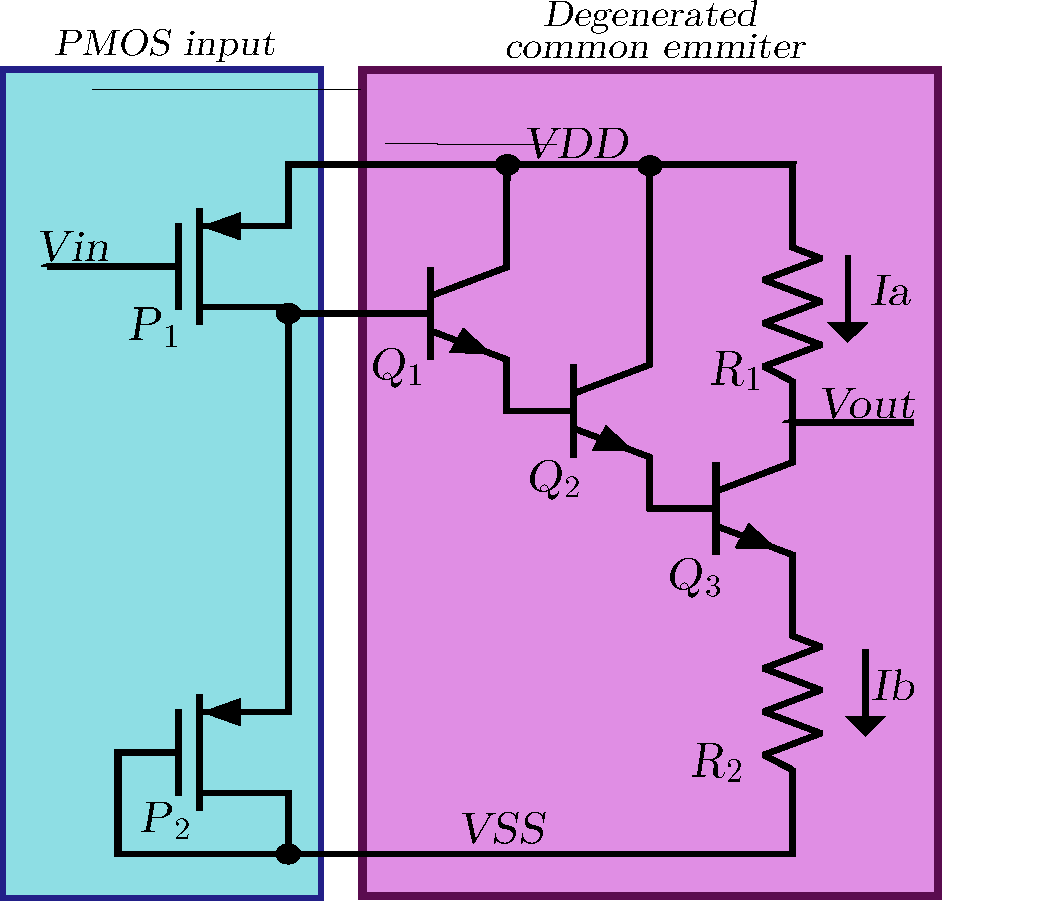
\includegraphics[width=0.5\textwidth]{audio002.pdf}
        \caption{audio002 amplifier schematic.}
        \label{audio002}
\end{figure}

\subsection{Circuit explanation}


This amplifier uses again a PMOS input in order to increase the input impedance of the amplifier. In order to increase the gain, a triple Darlington arrangement is used in order to increase the gain current and to improve temperature variations in comparison to a standard Darlington arrangement.

In this amplifier, in order to better define the initial operating point, the PMOS input stage is composed of two PMOS transistors: a current source PMOS ($P_2$) with its gate connected to $V_{SS}$, and an input PMOS with its gate connected to $V_{IN}$. This configuration ensures that the DC operating point is established through the relationship between the bias current of $P_2$ and the bias current of the base of $Q_1$.  

Since $P_2$ operates in saturation, the variation in current caused by a $\Delta V_{in}$ is primarily directed to the base of $Q_1$, so its essential to increase the $L$ of $P_{2}$ in order to reduce the channel modulation effect.

 A degeneration is putted  at the emitter of $Q_3$ in order to make the gain relation more linear and to increase the input impedance. The trade off is that the gain is smaller then a non-degenerated system, as the current gain will be naturally smaller.



Analyzing the circuit in the DC domain, first $V_{DD} -V_{IN} > V_{TH}$ in order for $P_1$ to be on, if not $V_{OUT} \approx V_{DD}$
Then the value of $V_{SD_{P2}}$ needs to be found, one to understand if $P_1$ is in saturation and to understand if $V_S{D_{P2}} > 3 \times 0.7$.
To start it is assumed $V_{SD_{P2}} >  3 \times 0.7$ and $V_{SG_{P1}}<V_{SD_{P1}}$, then

\[
    (V_{DD} - V_{IN} -VTH_{P1})^2 \times K_{P1}/2 = (V_{SD_{P2}} -VTH_{P2})^2 \times K_{P2}/2 + \frac{V_{SD_{P2}}}{(\beta_1+1) \times ((\beta_2 +1)(R_2 \times (\beta_3 +1) ))}.
\]

By solving this equation the value of $V_{SD_{P2}}$. If $V_{SD_{P2}} < 3 \times 0.7$ and $ V_{DD} - V_{IN} - Vth_{P1} < V_{DD} - V_{SD_{P2}}$, then

\[
    (V_{DD} - V_{IN} -VTH_{P1})^2 \times K_{P1}/2 = (V_{SD_{P2}} -VTH_{P2})^2 \times K_{P2}/2.
\]

And if $ V_{DD} - V_{IN} - Vth_{P1} > V_{DD} - V_{SD_{P2}}$ then 
\[
    (2 \times (V_{DD} - V_{IN}) \times V_{SD_{P1}} - V_{SD_{P1}}^2) \times K_{P1} = (V_{SD_{P2}} -VTH_{P2})^2 \times K_{P2}/2.
\]

Now assuming normal working conditions with $V_{SD_{P2}} > 3 \times 0.7$ and   $ V_{DD} - V_{IN} - Vth_{P1} < V_{DD} - V_{SD_{P2}}$, $IB_{Q3}$ can be expressed as

 \[
    IB_{Q3} = (\frac{V_{SD_{P2}}}{(\beta_1+1) \times ((\beta_2 +1)(R_2 \times (\beta_3 +1) ))} \times (\beta_1 + 1) ) \times (\beta_2 + 1).
\]

Since $IC_{Q3} = \beta_3 * IB_{Q3}$, $V_{OUT}$ can be expressed as


 \[
    V_{OUT} = V_{DD} - \beta_3 \times ((\frac{V_{SD_{P2}}}{(\beta_1+1) \times ((\beta_2 +1)(R_2 \times (\beta_3 +1) ))} \times (\beta_1 + 1) ) \times (\beta_2 + 1)).
\]



 The output impedance of the system is $R_1 || (R_{0Q3}+R_2)$

 Viewing the system in AC, in order to find the output transcondutance of the system, first the current gain of $P_1$ must be expressed.
 To better find the transcondutance its important to understand the equivalent emitter resistance in comparison to the driving signal. The emitter resistance can be broth up to the base by multiplying its value by $\beta$. Meaning in a small signal equivalent circuit, the equivalent resistance can be expressed approximately as $R_2 \times \beta_{Q1} \times \beta_{Q2} \times \beta_{Q3}$. Since the source of $P_2$ is connected to the node that varies with the total NPN current, the total transcondutance of the system can be expressed aproximatly as 
 
\begin{align}
   &\frac{-g_{mP1} \times \bigg(R0_{P1} \parallel  
   \bigg(\frac{1}{g_{mP2} + g_{mbP2} + \frac{1}{R0_{P2}}}\bigg) \parallel  
   \bigg((\beta_1+1) \times \big((\beta_2 +1)(R_2 \times (\beta_3 +1))\big)\bigg)\bigg)} 
   {(\beta_1+1) \times \big((\beta_2 +1)(R_2 \times (\beta_3 +1))\big)} \nonumber \\
   &\quad \times (\beta_1+1) \times (\beta_2 +1) \times \beta_3
\end{align}

Meaning the amplifier has a gain expressed as:

\begin{align}
    A_v \approx &\frac{-g_{mP1} \times \bigg(R0_{P1} \parallel  
    \bigg(\frac{1}{g_{mP2} + g_{mbP2} + \frac{1}{R0_{P2}}}\bigg) \parallel  
    \bigg((\beta_1+1) \times \big((\beta_2 +1)(R_2 \times (\beta_3 +1))\big)\bigg)\bigg)} 
    {(\beta_1+1) \times \big((\beta_2 +1)(R_2 \times (\beta_3 +1))\big)} \nonumber \\
    &\quad \times (\beta_1+1) \times (\beta_2 +1) \times \beta_3 \times \big(R_1 \parallel (R_{0Q3} + R_2)\big)
\end{align}





This is achieved by ignoring the the channel modulation effect of the MOS transistors and by ignoring other effects in the Bipolar transistors.



\begin{figure}[H]
        \centering
        \includesvg[width=1\textwidth]{audio002_ac_diagram.drawio.svg}
        \caption{audio002 amplifier block diagram.}
        \label{audio002_diag}
\end{figure}



\newpage



\section{audio003}

audio003 is a  two stage single input amplifier, exemplified in Fig. \ref{audio003}.
\begin{figure}[H]
        \centering
        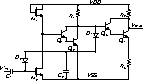
\includegraphics[width=0.7\textwidth]{audio003.pdf}
        \caption{audio003 amplifier schematic.}
        \label{audio003}
\end{figure}

\subsection{Circuit explanation}
Its based on this paper A Low Noise integratedUnibi Amplifier With Novel Biasing Scheme and Structure.
This is a two-stage amplifier that generates its own bias voltage through the DC feedback loop created by $D_1$ and $D_2$. Unfortunately, I could not implement this circuit using newer technologies (130 nm or 65 nm) the DC feedback loop doesn't work well with new technologies.  

The circuit operates by utilizing $C_1$ with the diodes in inversion. The diodes act as large resistances when reverse-biased, creating a high-pass filter that removes the DC and low-frequency noise components of $V_{in}$. The DC voltage is generated as the DC output of the first stage. Since the diodes draw almost no current, the gate DC voltage of $N_2$ is equal to the collector voltage of $Q_1$ and $Q_2$. Capacitor $C_2$ removes the AC component of the first stage at the gate of $N_2$, effectively acting as a low-pass filter.  

Assuming the DC operating point is fixed, all MOS transistors are in the saturation region, and all bipolar transistors are in the active region. When a variation in $V_{in}$ occurs, it induces a variation in the drain current of $N_2$. Since the current through $N_1$ remains relatively constant, the current shifts to $Q_1$. This current is further amplified by the Darlington configuration of $Q_2$, creating a current variation through $R_1$ approximately equal to
\[
-g_{mN2} \times \beta_1 - g_{mN2} \times \beta_1 \times \beta_2.
\]  

The total output impedance of the first stage can be expressed as
\[
R_1 \parallel R_{oQ2} \parallel (R_{oQ1} + R_{BEQ2}) \parallel \beta_3 \times \beta_4 \times R_3.
\]  

Since it is assumed that $R_3$ is significantly larger than the base-emitter resistance, $R_3$ multiplied by the $\beta$ values of $Q_3$ and $Q_4$ dominates the equivalent emitter resistance. 

Giving a gain of the first stage equal to

\begin{equation}
    A_v = (-g_{mN2} \times \beta_1 - g_{mN2} \times \beta_1 \times \beta_2) \times (R_1 \parallel R_{oQ2} \parallel (R_{oQ1} + R_{BEQ2}) \parallel( \beta_3 \times \beta_4 \times R_3)).
\end{equation}

The base current variation of $Q_3$ (again ignoring the base-emitter resistance) can be expressed approximately as:  
\[
\frac{\Delta V_{\text{out1stage}}}{(\beta_3 + 1) \times (\beta_4 + 1) \times R_3},
\]  
which results in a total variation through $R_2$ of approximately:  
\[
\frac{\Delta V_{\text{out1stage}}}{((\beta_3 + 1) \times (\beta_4 + 1) \times R_3)((\beta_3 + 1) \times \beta_4)}.
\]  

The output impedance of the second stage can be expressed as:  
\[
R_2 \parallel \left(R_3 + \left(R_{oQ4} \parallel \left(R_{oQ4} + R_{BEQ2}\right)\right)\right),
\]  
making the gain of the second stage:  
\[
A_v = \frac{R_2 \parallel \left(R_3 + \left(R_{oQ4} \parallel \left(R_{oQ4} + R_{BEQ2}\right)\right)\right)}{((\beta_3 + 1) \times (\beta_4 + 1) \times R_3)((\beta_3 + 1) \times \beta_4)}.
\]





\begin{figure}[H]
        \centering
        \includesvg[width=1\textwidth]{audio003_ac_block.drawio.svg}
        \caption{audio003 amplifier block diagram.}
        \label{audio003_diag}
\end{figure}



\newpage

\section{AGC1}

AGC1 is a  two stage single input amplifier, exemplified in Fig. \ref{audio004}. 
\begin{figure}[H]
        \centering
        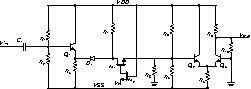
\includegraphics[width=1\textwidth]{audio004.pdf}
        \caption{AGC001 amplifier schematic.}
        \label{audio004}
\end{figure}
\subsection{Circuit explanation}
Now this is amplifier with a gain control mechanism in the form of $V_C$. It is based on a very old paper, A Wide-Band AGC Block Suitable fo’r Integrated Realization. 

To start off, $C_1$ is a decoupling capacitor forming a high-pass filter to remove the DC component of $V_{IN}$. The relationship between $R_1$ and $R_2$ defines the bias point of $Q_1$. Resistor $R_3$ is chosen such that $R_3 \times \beta_1$ is much larger than $R_2$, minimizing the loading effect and keeping the bias point as close as possible to:  
\[
\frac{(V_{DD} - V_{SS}) \times R_1}{R_1 + R_2}.
\]  

Due to the inherent voltage drop of a common-collector amplifier (which is very close to the voltage drop of a diode, as both involve a PN junction), a diode is placed to ensure the left-side voltage of $N_1$ remains approximately equal to $V_{IN}$. This technique is commonly used in older bipolar circuit designs, particularly in simpler buffer circuits.

Now, $R_4$ serves the purpose of providing current to the left side of $N_1$. $N_1$ operates in the triode region, functioning as a controllable resistor dependent on the value of $V_C$, enabling attenuation to be controlled. Depending on the value of $V_C$, the attenuation varies: higher resistance results in greater attenuation, while lower resistance results in less attenuation.

The second stage is an unconventional differential pair configuration, where $R_8$ serves as the biasing mechanism for the differential pair. Since the differential pair is uncompensated and the $V_{BE}$ of $Q_3$ is always equal, the circuit essentially exhibits a positive gain relative to the input. The ratio between $R_3$ and $R_8$ controls the DC point of $V_{out}$. $R_6$ and $R_7$ define a theoretical DC point at the input of the second stage, but the lack of a decoupling capacitor significantly degrades the circuit. The addition of a decoupling capacitor greatly improves this circuit by isolating the actual DC points.

This circuit suffers significantly from offset. However, offset does not seem to have been a critical concern in these older circuits, many of which perform poorly compared to modern designs.  

A version of this circuit was implemented in LTspice using actual JFET transistors to mimic the paper design. In comparison to the paper, this amplifier functions as more than just a controllable attenuator. The amplifier works, and its gain is effectively controlled by $V_C$. It achieves a relatively good FFT performance for its type, although the FFT degrades as the gain decreases, which is due to the characteristics of JFET operation.




\newpage




\section{PDM001}


PDM001 is a power switch driver for motor aplications Fig. \ref{PDM001}. 

\begin{figure}[H]
        \centering
        \includesvg[width=0.4\textwidth]{PDM_driver.drawio.svg}
        \caption{PDM001 driver schematic.}
        \label{PDM001}
\end{figure}


\subsection{Circuit explanation}

This is a primordial power circuit for integrated circuits intended for power applications. As with many primordial circuits, it is not particularly effective; however, it is a fun circuit to analyze.  
A version of this circuit was implemented in LTspice.  

It is based on the paper *Semiconductor Networks for Linear Amplification Using the Switching Mode*.  

This is a solely bipolar circuit that can be implemented in a bipolar-only process. It works by inputting a positive and negative square wave at its input. If the input is positive, the upper switch is activated; if negative, the second switch is activated.  

This circuit uses $V_{DD}$ as the positive supply, $V_{SS}$ as the negative supply, and ground as the reference. When the input voltage is positive, $Q_1$ has a positive $V_{BE}$ potential, meaning it is turned on. For $Q_1$ to operate in saturation, its collector voltage must be as close to $0 \, \text{V}$ as possible, with $V_{CE}$ around $100 \, \text{mV}$. Thus, the value of $R_1$ should be chosen relatively high to achieve this.  

Another important factor is the negative $V_{SS}$. The negative $V_{SS}$ constrains the maximum input signal, for example, to approximately $1 \, \text{V}$. This ensures that the emitter voltage of $Q_1$ remains close to $0.3 \, \text{V}$ and the collector voltage of $Q_1$ is also close to $0.3 \, \text{V}$, as $Q_1$ is saturated. However, because $V_{SS}$ is negative, this $0.3 \, \text{V}$ is sufficient to bias $Q_4$. The value of $R_5$ is then used to control the current flow through the circuit.  

Since the $V_C$ of $Q_1$ is very close to $0 \, \text{V}$, the base-emitter voltage of $Q_2$ is insufficient to turn it on, keeping $Q_2$ in the off state. As a result, the collector voltage of $Q_2$ is close to $V_{DD}$, causing $Q_3$ to turn on. This makes $V_{\text{OUT1}}$ equal to $V_{DD} - 0.7 \, \text{V}$, meaning the power switch associated with $Q_3$ is activated.  

Meanwhile, the collector voltage of $Q_4$ is either below or very close to $0 \, \text{V}$, ensuring that $Q_5$ remains off, and consequently, $V_{\text{OUT2}}$ is $0 \, \text{V}$.  

When $V_{\text{in}}$ is a negative voltage, $Q_1$ turns off because it has a negative $V_{BE}$ voltage. This results in a collector voltage close to $V_{DD}$, turning $Q_2$ on. Consequently, $Q_3$ turns off, and $V_{\text{OUT1}}$ becomes close to $0 \, \text{V}$.  

On the lower side, the $V_{BE}$ of $Q_4$ is insufficient to turn it on, leaving $Q_4$ in the off state. Consequently, its collector voltage is close to $V_{DD}$, turning $Q_5$ on. This makes $V_{\text{OUT2}}$ equal to $V_{DD} - 0.7 \, \text{V}$, activating the second power switch.

This circuit is relatively amusing to analyze and size, but it is not particularly effective due to the significant disadvantages of bipolar switches compared to FET switches. While the bipolar switches are not explicitly shown in the schematic, they are included in the LTSpice implementation and are present in the original paper.  

To properly size this circuit, it is crucial to understand the relationship between the value of $V_{\text{IN}}$ and its effects on the various nodes. Notably, $D_5$ introduces a specific influence on the $V_{\text{OUT2}}$ voltage when $V_{\text{IN}}$ is negative.  


\newpage


\section{BIstable001}



bistable001 is a bi stable circutit shown in Fig. \ref{bistable001}. 

\begin{figure}[H]
        \centering
        \includesvg[width=0.4\textwidth]{bi_stable_circuit001.drawio.svg}
        \caption{bistable001 driver schematic.}
        \label{bistable001}
\end{figure}

\subsection{Circuit explanation}

A version of this circuit was implemented in LTspice.  
Based on this paper A simple integrated realization of a new bistable circuit.

This is a bistable circuit with a memory component. The memory component of this circuit is the $RC$ network composed of $R_2$ and $C_1$.  

This circuit operates in two distinct states, which can be toggled by a sudden variation in $V_{\text{IN}}$. Such a change induces and forces the bistable circuit to switch states.  

Starting with the initial state of the circuit, $Q_1$ is biased because its $V_{\text{BE}}$ exceeds $0.7 \, \text{V}$. This causes current to flow through the emitter, which equals the $I_{\text{D}}$ of $P_1$ (a PJFET). Consequently, $V_{\text{OUT}}$ settles at the voltage where its current matches the emitter current of $Q_1$, requiring it to be a negative voltage close to the $V_{\text{SS}}$ rail.  Now because if the network $R_2$ and $C_1$, the voltage of the base of $Q_1$ will be close to $V_{OUT} + 0.7$(in order for the voltage $V_{BE}$ voltage of $Q_1$ to be larger then 0.7).

When a fast switching event occurs at $V_{\text{IN}}$ (from example -2 to 2 Volts), a current is injected at the drain of $P_1$. This causes the $V_{\text{DS}}$ of $P_1$ to experience a voltage variation.  

This voltage variation forces $Q_1$ to shut off, reducing its emitter resistance to nearly zero. Consequently, $V_{\text{OUT}}$ approaches $V_{\text{DD}}$, and $P_1$ shuts down. It is important to note that the injected current resembles a pulse due to the presence of the input capacitor.  

When the variation transitions from a positive to a negative value, the opposite occurs. A current is forced through ground, passing through $R_2$ into the base-emitter junction of $Q_1$, and then through $C_2$. This process forces $Q_1$ to turn on, thereby restoring the circuit to its original working state.  


The amusing aspect of this circuit is that its operation is controlled by the switching velocity and the magnitude of the voltage change, which is converted into an input current pulse through $C_2$.  

If the voltage switching occurs too slowly, the circuit will fail to switch states and will remain in its saved state. This behavior makes it a rather unusual memory circuit.  

As with the previous circuits, it is not particularly practical or useful. However, it is an interesting design as it helps in exploring different circuit concepts.






\newpage


\section{analog switch01}



analog switch01 is a FET driven switch with a bipolar driver circuit shown in Fig. \ref{analogswitch01}. 

\begin{figure}[H]
        \centering
        \includesvg[width=0.4\textwidth]{analog_switching_circuit.drawio.svg}
        \caption{analog switch01 schematic.}
        \label{analogswitch01}
\end{figure}

\subsection{Circuit explanation}
This circuit is based on the paper *An Integrated FET Analog Switch*.  
As with the other circuits, a version has been implemented in LTspice.  

This circuit is relatively simple. The driver consists of a PNP transistor, $Q_1$, the current-limiting resistors $R_1 - R_3$, the biasing capacitor $C_1$, the blocking diode $D_1$, and an NJFET, $N_1$.  

When $V_{\text{in}}$ is negative (as PNP uses inverse logic), the $V_{\text{EB}}$ of $Q_1$ is biased, causing $Q_1$ to drive a current. Most of this current flows through $R_1$, while a portion flows through $C_1$, which biases the gate capacitance of $N_1$, turning it on. The capacitor $C_1$ and the diode $D_1$ serve protective roles for $N_1$: the capacitor ensures no DC current flows into the FET, and the diode removes the gate charge when the FET turns off. These components are unnecessary when using an NMOS device.  

When $V_{\text{in}}$ transitions to a positive voltage close to $V_{\text{DD}}$, $Q_1$ turns off, causing the collector voltage of $Q_5$ to equal $V_{\text{SS}}$. During the switch-off process, $D_1$ discharges the gate capacitance of $N_1$, bringing the gate voltage below $V_{\text{SS}}$, and $N_1$ turns off.  


\newpage
\section{Bipolar buffer1}



Bipolar buffer1 is a two stage differential bipolar amplifier in buffer configuration in Fig. \ref{bipolarbuffer01}. 

\begin{figure}[H]
        \centering
        \includesvg[width=0.4\textwidth]{Bipolar_buffer_1.drawio.svg}
        \caption{Bipolar buffer1  schematic.}
        \label{bipolarbuffer01}
\end{figure}

\subsection{Circuit explanation}


Again it's a primordial integrated differential amplifier. This time is not based on any paper.

To start off, assuming that $V_{\text{IN+}}$ is the input signal of $Q_1$ and that $Q_2$'s base is not connected to the amplifier output but instead connected to an arbitrary $V_{\text{IN-}}$ signal, it is assumed that both $V_{\text{IN}}$ signals have an equal DC component.

In this circuit, $R_1$ serves the purpose of creating a collector voltage variation at the collector terminal of $Q_1$, which is in a differential pair configuration with $Q_2$. $R_2$ serves as the current bias generator of this circuit, where the bias current can be expressed as  
\begin{equation}
    I_{\text{Bias}} = \frac{V_{\text{IN}_{\text{DC}}} - 0.7}{2 \beta_{1} \times R_2},
\end{equation}  
where $\beta_1 = \beta_2$ and $0.7$~V is the $V_{\text{BE}}$ required to bias the bipolar transistors.  

Assuming a state where both collector currents are equal (they are not in reality because $V_{\text{CE}}$ of both $Q_1$ and $Q_2$ is different, causing some offset current), the bias setpoint of the output of the first stage can be defined as  
\[
V_{DD} - \frac{I_{\text{Bias}}}{2} \times R_1.
\]  
Due to the next stage, this voltage, as a rule of thumb, needs to be lower than $V_{\text{DD}}$ by a value larger than $0.7$~V in order to bias $Q_3$, which is a PNP bipolar transistor.  

Regarding $R_3$, to minimize its input impedance, the condition $R_3 \cdot \beta_3 \gg R_1$ must hold. The collector current of $Q_3$, $I_{\text{CQ3}}$, equals  
\[
I_{\text{CQ3}} \approx  \frac{V_{\text{DD}} - 0.7 - V_{\text{CQ1}}}{R_3}.
\]  

Then, $R_4$ should be defined so that  
\[
\beta_3 \times \frac{V_{\text{DD}} - 0.7 - V_{\text{CQ1}}}{R_3} \times R_4
\]  
equals the desired $V_{\text{OUT}_{\text{DC}}}$ value.  


Assuming that in the DC state all transistors are in the amplification stage, when a variation appears at $V_{\text{IN+}}$, it causes a current variation in $Q_1$'s collector current equal to $\beta_1 \times \frac{\Delta V_{\text{IN+}}}{R_2}$, where $g_{mQ_1} \approx \frac{\beta_1}{R_2}$.  

Since the current flowing through is assumed even though it is not accurate in this configuration (the largest problem of using resistors as current sources instead of transistors), the impedance of the first stage can be expressed as  
\[
R_1 \parallel R_{0Q_1} \parallel R_3 \cdot \beta_3,
\]  
and the gain of the first stage is expressed as  
\[
-g_{mQ_1} \cdot \left( R_1 \parallel R_{0Q_1} \parallel R_3 \cdot \beta_3 \right).
\]  

In the second stage, the transconductance can be expressed as $\beta_3 \cdot \frac{\Delta V_{\text{in}}}{R_3}$, where $g_{mQ_3} = \frac{\beta_3}{R_3}$. The gain of the second stage can be expressed as  
\[
-g_{mQ_3} \cdot \left( (R_3 + R_{0Q_3}) \parallel R_4 \right).
\]  

By multiplying the gains of the two stages, the overall gain of the amplifier can be expressed as  
\[
g_{mQ_1} \cdot \left( R_1 \parallel R_{0Q_1} \parallel R_3 \cdot \beta_3 \right) \cdot g_{mQ_3} \cdot \left( (R_3 + R_{0Q_3}) \parallel R_4 \right).
\]  



\begin{figure}[H]
        \centering
        \includesvg[width=1\textwidth]{BIpolar_buffer_diagram.drawio.svg}
        \caption{Bipolar buffer1  diagram block.}
        \label{bipolarbuffer01dig}
\end{figure}








Since almost all two-stage amplifiers are unstable, a capacitor, $C_1$, is used to slow down the first stage and essentially make the amplifier stable. In control terms, it increases the distance between the two dominant poles.


A prototype was made in LTspice in the repository. Another was made in TSMC180BCD process using power bipolars transistors.






\newpage

\section{Bipolar buffer2}



Bipolar buffer2 is a two stage differential bipolar amplifier in buffer configuration in Fig. \ref{bipolarbuffer02}. 

\begin{figure}[H]
        \centering
        \includesvg[width=0.4\textwidth]{Bipolar_buffer2.drawio.svg}
        \caption{Bipolar buffer2  schematic.}
        \label{bipolarbuffer02}
\end{figure}

\subsection{Circuit explanation}

This is an improvement of the previous amplifier presented in the paper *"An Integrated Buffer Amplifier"*.  

In this differential pair, it is composed of two Darlington NPN configurations that are used to increase the input impedance of the differential pair. Again, the differential pair is biased by a resistor. The $I_{\text{BIAS}}$ can be calculated as  
\[
I_{\text{BIAS}} = \frac{V_{\text{IN}} - 2 \times 0.7}{R_3},
\]  
where, again, because of the resistor, the bias current is always dependent on the DC point of $V_{\text{IN,DC}}$.  

The DC point of the first stage can be calculated as  
\[
V_{\text{DD}} - \frac{I_{\text{BIAS}}}{2} \cdot R_1 - 0.7.
\]  

In this case, to reduce current mismatch between the differential pair caused by the forward voltage effect of the bipolar transistors, both pairs include a resistance of the same value. To better compensate for temperature variation, one diode is implemented. This diode introduces a voltage drop without needing to increase the current but effectively reduces the gain because the resistance value must be decreased to make the DC point relatively large.  

The AC gain can be calculated as  
\[
-g_{mQ_1Q_3} \cdot \left( R_1 \parallel R_{0Q_3} \parallel R_4 \cdot \beta_5 \right),
\]  
where  
\[
g_{mQ_1Q_3} \approx \beta_1 \cdot \beta_3 \cdot \frac{1}{R_3}.
\]

In relation to the second stage, to improve its characteristics, two diodes are implemented in series. This is done to compensate for the voltage drops caused by the two PN junction voltage drops of the Darlington configuration and to improve temperature stability.  

By including these diodes, $V_{\text{OUT}}$ becomes more stable, but the gain of the amplifier is smaller compared to its version without the diodes. However, this design significantly reduces the amplifier's DC offset as a function of temperature, since the variation of the diodes is relatively equal to the variation of the bipolar transistors, in comparison to the resistance variance with temperature.  

The AC gain of the second stage is essentially equal to the AC gain of the previous amplifier's second stage.
And the gain of this amplifier can be expressed as  

\[
g_{mQ_1Q_3} \cdot \left( R_1 \parallel R_{0Q_3} \parallel \left( R_4 \cdot \beta_5 \right) \right) \cdot \beta_4 \cdot g_{mQ_4} \cdot \left( \left( R_4 + R_{0Q_4} \right) \parallel R_5 \right).
\]


It is important to note that the first integrated monolithic operational amplifier (OPAMP) was made in 1963. This paper is from 1965. Therefore, in this sense, these are early monolithic amplifier designs, and it is normal that they do not perform well when used with today’s processes, and where at the time the stepping stones to the designs we have today.  

This amplifier was implemented in LTSPICE and the TSMC180BCD process. The LTSPICE design is publicly available in the repository.

\newpage

\section{RF001}



RF001 bipolar TV receiver circuit in Fig. \ref{RF001 }. 

\begin{figure}[H]
        \centering
        \includesvg[width=1\textwidth]{tv_receiver.drawio.svg}
        \caption{RF001   schematic.}
        \label{RF001 }
\end{figure}

\subsection{Circuit explanation}

RF001 is one of the first integrated RF circuits. It was designed for use in old TV receivers.  

It is based on the paper *INTEGRATED CIRCUITS IN TELEVISION RECEIVERS*. Without delving too much into the theory, the sound band carrier (41.25 MHz) and the picture wave carrier (45.75 MHz) are multiplied by each other (frequency modulated beat) to generate a lower frequency sinusoidal wave centered at 4.5 MHz. This 4.5 MHz sinusoidal wave is considered the input wave.  

Generally speaking, these modulated waves have a very low amplitude and need to be amplified for further processing. In simple terms, this circuit amplifies the sinusoidal wave and shifts it by 90 degrees (quadrature) for subsequent processing.

A design was made in LTspice and in TSMC180BCD process, generally doing bipolars in LTspice is far easier because of their higher $\beta$ compared to lateral bipolar in CMOS process. But doing circuits in virtuoso is far easier then in LTspice.

To start off, the first part of the circuit involves the power management area composed of $D_1 - D_7$, $R_9$, $R_{10}$, $Q_9$, and $Q_{10}$.  

In simple terms, the main $V_{DD}$ is too large, and in order to reduce it and generate other voltage references for the circuit, this section is used. To begin, a resistor in conjunction with the seven diodes is used to fix the base voltage of $Q_9$. Assuming each diode requires a voltage of 0.7 V and $R_9$ has a low value, the base voltage of $Q_9$ can be approximated as 4.9 V.  

Because of the base-emitter junction of $Q_9$, this produces a reference current of approximately 4.2 V. The reference should be designed such that its value does not significantly change with consumption. To achieve this, a low value for $R_9$ is required.

For the reference voltage, the same principle applies. Because the reference has four diodes, the base voltage will be approximately 2.8 V. Due to the inherent base-emitter voltage drop of all bipolars, this will generate a bias voltage of approximately 2.1 V.  

In this case, $R_{10}$ needs to be relatively large in order to increase the input impedance of this stage, as this transistor itself will not be driving a large load.

Starting with the first amplifier of the amplifying chain, it is composed of $Q_1$, $Q_2$, $Q_3$, $R_1$, $R_2$, and $R_3$. Essentially, it is a two-stage amplifier with a differential stage and an output stage.  

Because it does not include the usual slewing stage, the first stage operates as a non-inverting stage, meaning the output is directly proportional to the output stage. This explains why the resistor is connected to the inverting input of the amplifier.



To start, $V_{IN+}$ is DC biased by the reference voltage, and the AC input signal is coupled to a transistor. For this system to work properly, the DC voltage of $V_{IN-}$ must be very close to the DC value of $V_{IN+}$, and the output voltage of the second stage should also be very close to $V_{IN+DC}$.  

To achieve this, $R_2 = 2 \cdot R_1$, and $R_3$ is chosen to be relatively high to increase the input impedance of $Q_3$. This configuration produces a voltage at $V_{C_{Q_2}}$ that is very close to $V_{IN+DC} + 0.7$. By applying the common collector stage, this $0.7$ V offset is removed, making the DC output very close to the input DC value.  

Of course, this comes at the cost of a lower AC gain, but it is a trade-off that improves DC performance.

For simplicity reasons the ac gain of the second stage is considered 1, so the ac gain of this stage can be considered equal to
\[
    A_v = R_2 \parallel R0_{Q2} \times \frac{\beta_1}{1 + \beta_1\times R_1}
 \]


The second stage is exactly the same as the first stage, with its output connected to the inverting input of the first stage. However, it is filtered through a low-pass filter to remove the AC component from the feedback loop. As stated before, the output will be very close to the input due to the resistor relationship. 

There will be a slight difference because of the forward voltage phenomenon, but the variation will only be a few millivolts. Once again, the gain of this stage will be equal to the gain of the previous stage. The inverse input of this amplifier is equal to the voltage reference, that is exactly close to 2.1 V.

Next is the final amplification stage, that is just a differential pair with an inductive load. again in this differential pair, $Q_8$ is connected again to the voltage reference that is 2.1.

What this does is that the voltage gain is converted into a current variation through $I_{C_{Q_8}}$. Since its collector current is directly connected to a phase shift transformer, this will induce the same current variation in the secondary part of the transformer but shifted by 90° (in quadrature). 

The secondary middle is connected to the voltage reference, meaning the DC current is biased. While the mutual inductance is not specified, theoretically this current variation will be input into the degenerated Darlington configuration, generating a current. 
The second part is a FM detector, basicly is a frequency to voltage converter, with diodes actinas capacitors.

This part could not be implemented correctly in LTspice or in Virtuoso.



\begin{figure}[H]
        \centering
        \includesvg[width=1\textwidth]{RF001_AC_DIAGRAM.drawio.svg}
        \caption{RF001 block diagram schematic.}
        \label{RF001block }
\end{figure}

\newpage



\end{document}
